%!TEX root = ../main.tex
%%%%%%%%%%%%%%%%%%%%%%%%%%%%%%%%%%
% Links:
%
% Difficulty:
% Companies: 
%%%%%%%%%%%%%%%%%%%%%%%%%%%%%%%%%%


%\begin{figure}
%	\centering
%	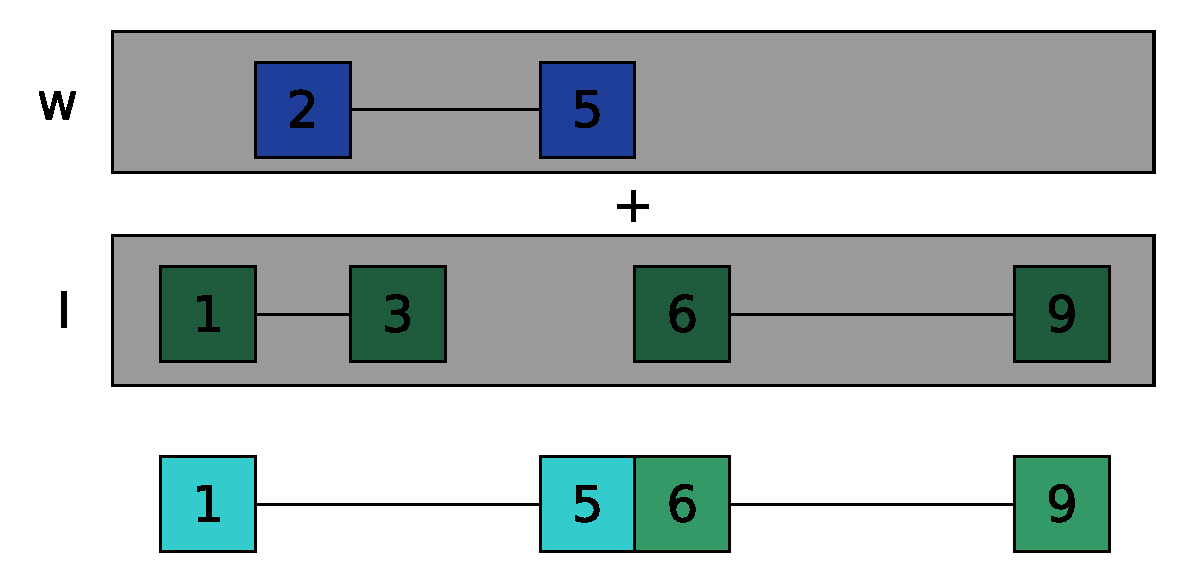
\includegraphics[width=\textwidth]{sources/merge_intervals_2/images/example1}
%	\caption[Sample short cpation]{Sample Caption}.
%	\label{fig:merge_intervals_2:example1}
%\end{figure}

\chapter{Merge Intervals}
\label{ch:merge_intervals_2}
\section*{Introduction}
Intervals are common in programming and they pop up in numerous applications as they are very versatile and are used to represent many things, from finite segments in a gemoetry application to time spans for a school timetable.

Intervals are also quite popular in interview questions; In this chapter will go through one that is commonly asked (still nowadays) at Google where we are given a list of time intervals and we need to produce a new list where none of the elements overlap with one another.

In addition, we will also investigate, in Section \ref{example:merge_intervals_2:exercice1_2}, a variation of this problem where we are given a list of time intervals where we are guaranteed none of them overlaps wtih one another to begin with and our job is to insert a new interval in the list in such a way that the non-overlapping property is maintained.

\section{Problem statement}
\begin{exercise}
\label{example:merge_intervals_2:exercice1_1}
Write a function that, given a list of intervals $I=\{(s_0, e_0),(s_1, e_1), \ldots,(s_{n-1}, e_{n-1})\}$ represented as a pair of integers, returns a new list $I'$ which is a copy of $I$ except that overlapping intervals are merged together. 
The resulting list should only contain non-overlapping intervals.

	%example1
	\begin{example}
		\label{example:merge_intervals_2:example1_1}
		\hfill \\
		Given $I=\{(3, 7),(1, 5), (6, 8),(4, 6)  \}$ returns $I'=\{(1,8)\}$.
	\end{example}

	\begin{example}
		\label{example:merge_intervals_2:example1_2}
		\hfill \\
		Given $I=\{(1, 5), (6, 7), (4, 4), (9, 12) \}$ returns $I'=\{(1,5),(6,7),(9,12)\}$.
	\end{example}
\end{exercise}

\section{Clarification Questions}

\begin{QandA}
	\begin{questionitem} \begin{question} (If not clear from the examples) Is it guaranteed for the intervals to be sorted? (either by the starting or ending time of the interval) \end{question} 	 
    \begin{answered}
		\textit{No, the input is not sorted.}
	\end{answered} \end{questionitem}

	\begin{questionitem} \begin{question} Can the input list be modified?\end{question} 	 
    \begin{answered}
		\textit{No, $I$ is read-only.}
	\end{answered} \end{questionitem}

	\begin{questionitem} \begin{question} Can we always assume that given an interval $(x,y)$ in $I$, $ x \leq y$ always holds?\end{question} 	 
		\begin{answered}
			\textit{Yes individual intervals have the first component always smaller or equal than the second.}
		\end{answered} \end{questionitem}
\end{QandA}


\section{Discussion}
\label{example:merge_intervals_2:discussion_1}
Let's have a closer look at why Example \ref{example:merge_intervals_2:example1_1} results in $I'=\{(1,8)\}$.
Intervals $(3,7)$ and $(1,5)$ overlap and they can be merged into $(1,7)$ which can in turn, be merged with both $(6,8)$ and $(4,6)$.
Because $\{(4,6)\}$ lies completely inside $(1,7)$, merging them results still in $(1,7)$.
Finally, $\{(1,7)\}$ also overlaps with $(6,8)$ and blending the two of them together yields $\{(1,8)\}$.

We can determine if two intervals $a=(a_s,a_e)$ and $b=(b_s,b_e)$ overlap if any of the following is true:
\begin{itemize}
	\item $a$ is fully contained in $b$: this happens when both $a_s$ and $a_e$ are within $b$ i.e. $a_s \geq b_s$ and   $a_e \leq b_e$ e.g. $(10,19)$ is fully contained in $(9,20)$;
	\item $b$ is fully contained in $a$;
	\item $a_s$ is partially contained in $b$ i.e. $a_s \geq b_s $ and $a_s \leq b_e$.
	\item $b_s$ is partially contained in $a$ i.e. $b_s \geq a_s $ and $b_s \leq a_e$.
\end{itemize}
If none of the above condition is met then $a$ and $b$ are completely disjoint.

\subsection{Brute-Force}
\label{example:merge_intervals_2:bruteforce_1}
We can use these facts to build a solution that examines one interval at the time, starting from the first one and greedily tries to merge it with as many other intervals as possible.
The idea is that once we picked an interval $x$ we will merge it with all the other overlapping intervals. 
This results in a interval $m$ which is the combination of $x$ and zero or more other intervals in the list.
We can at this point add $m$ to the output list. We can also mark the intervals we merged $x$ with, so that they will be ignored for the remainder of the process: after-all they are already accounted for in $m$.
If we repeat this process for each and every unmarked interval of $I$ we will eventually have an output list $I$ that contains only un-mergable and non-overlapping intervals. 
This idea is implemented in Listing \ref{list:merge_intervals_2_bruteforce}. 

\lstinputlisting[language=c++, caption={Quadratic time solution.},label=list:merge_intervals_2_bruteforce]{sources/merge_intervals_2/merge_intervals_2_merge_entire_list_solution2.cpp}

The function \inline{merge} contains the logic for merging two intervals and it is used in the main function \inline{merge_list_intervals_entire_list_bruteforce} that loops through the elements of the input list one at the time and carefully uses an array of boolean flags \inline{excluded} to mark intervals that have been already merged.
If an interval is not yet merged into the output list \inline{ans} then we place it at the back of \inline{ans} and then we try to merge it with the rest of the unmarked intervals (in the innermost loop).
Whenever it overlaps with some other interval the resulting merged interval is substituted at the back of \inline{ans} and the interval it was merged with is marked as to be excluded from further examination in the future iterations.
Therefore each and every interval is either used as a starting seed and is tested for overlap and potentially merged with the remaining of the not yet excluded intervals or, it is skipped altogether because was already merged in a previous iteration.
Notice that the inner loop starts at $j=i+1$ as intervals before position $i$ have been already merged (and clearly we do not need to test for overlapping when $i=j$).

Using this strategy, we are sure that the output list will never contain any interval that is not covered by one or more intervals in the input list. 
Similarly, if a value is covered by an interval in $I$ then, we are also guaranteed it will be contained in the output.
In other words, if you imagine that a list of intervals represent colored segments of a line then $I$ and $I'$ would produce the very same exact coloring of the line.

The complexity of this function is quadratic in time; when we have an input list containing only non-overlapping intervals, none of them (except the one we are trying to merge the others with) will ever be excluded and that means a full run of the innerloop will occur.

The space complexity is linear as we use an array of the same size of $I$ for the output list as well as for the array of flags \inline{excluded}. 

\subsection{$nlog(n)$ sorting solution}
\label{example:merge_intervals_2:sorting_1}
The quadratic solution presented in Section \ref{example:merge_intervals_2:bruteforce_1} is correct but it does quite a lot of unnecessary work.
When we start examining an not yet excluded interval at index $i$ we are forced to take a look at all the other subsequent intervals in the list because we have no way of knowing whether there will be one with which interval $i$ overlaps with.
However, \textbf{this is not true if the intervals are sorted}. 
Let's assume $I$ is sorted by the $start$ field and that ties between intervals (intervals starting at the same value) are resolved using the $end$ field.
When examining the interval $I_i$ we can simply look at the next interval $I_{i+1}$ and if it does not overlap with $I_i$ then we are sure that none of the elements ahead of it will!
The reason is that in order for interval $I_i$ not to overlap with $I_{i+1}$ it has to be that $I_i.end < I_{i+1}.start$.
Because intervals are sorted by their $start$ fields, any subsequent intervals will have an even higher $start$ value. 
This allows us to save tons of work as we can merge the entire list in linear time once it is sorted. 

Listing \ref{list:merge_intervals_2_nlogn} implements this idea.

\lstinputlisting[language=c++, caption={$nlog(n)$ time solution using sorting.},label=list:merge_intervals_2_nlogn]{sources/merge_intervals_2/merge_intervals_2_merge_entire_list_solution1.cpp}

Not surprisingly the first thing this code does is sorting the input list.
We then start by pushing the first interval into the output list \inline{ans}.
We keep merging subsequent elements that overlap with \inline{ans.back} until we find one that does not.
At this point we are sure that whatever interval is in \inline{ans.back} will definitely not overlap with any other interval in the list.
Therefore we can safely push this new interval into \inline{ans} and repeat the process until all intervals have been analyzed.

Notice that here we are using the same \inline{merge} function used in Listing \ref{list:merge_intervals_2_bruteforce};
However, because we know elements are sorted we could simplify the condition \inline{if ((a.start >= b.start && a.start <= b.end) || (b.start >= a.start && b.start <= a.end))} as we know that \inline{a.start <= b.start} is always true.

This approach has a time complexity of $nlog(n)$ (due to the sorting) 
and the space complexity is $O(n)$ (however we really only use linear spcae to store the output list and if we do not account for it the complexity is constant).

\section{Problem statement}
\begin{exercise}
\label{example:merge_intervals_2:exercice1_2}

Given a sorted list of disjoint (non-overlapping) intervals $I$ and an interval $w$, insert $w$ into $I$ so that the resulting list still contains only disjoint intervals.
You may assume that the intervals are sorted according to their start times.

	%example1
	\begin{example}
		\label{example:merge_intervals_2:example1}
		\hfill \\
		Given $I=\{(1,3),(6,9)\}$ and $w=(2,5)$ the function returns $I'=\{(1,5),(6,9)\}$ (see Figure \ref{example:merge_intervals_2:example1}).
	\end{example}

	%example2
	\begin{example}
		\label{example:merge_intervals_2:example2}
		\hfill \\
		Given $I=\{(1,2),(3,5),(6,7),(8,10),(12,16)\}$ and $w=(4,9)$ the function returns $I'=\{(1,2),(3,10),(12,16)\}$
	\end{example}

\end{exercise}

\begin{figure}
	\centering
	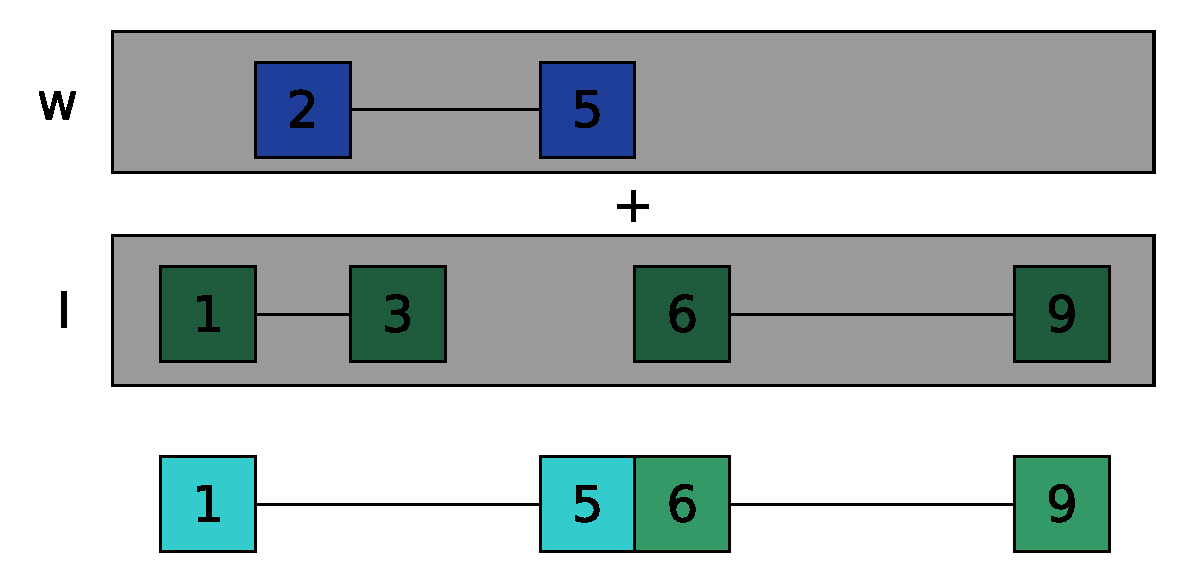
\includegraphics[width=\textwidth]{sources/merge_intervals_2/images/example1}
	\caption[Implicit graph for the Example \ref{example:merge_intervals_2:example1}.]
	{Visual representation the problem instance of Example
	\ref{example:merge_intervals_2:example1}.The \textcolor[HTML]{339966}{$\blacksquare$} green $(1,3)$ and \textcolor[HTML]{3366ff}{$\blacksquare$} blue interval $(2,5)$  are merged together into the \textcolor[HTML]{33cccc}{$\blacksquare$}cyan interval $(1,5)$ (in the bottom row). The interval $(6,9)$ in $I$ does not overlap with either $(2,5)$ not with newly formed $(1,5)$ and it is therefore simply copied over to the answer list.}
	\label{fig:merge_intervals_2:example1}
\end{figure}


\FloatBarrier

\section{Discussion}
\label{merge_intervals_2:sec:discussion_1}


\subsection{Brute-force}
\label{merge_intervals_2:sec:bruteforce_1}

\lstinputlisting[language=c++, caption={Linear time solution.},label=list:merge_intervals_2]{sources/merge_intervals_2/merge_intervals_2_solution1.cpp}

